\section{Ejemplo con una pecera}

\begin{center}
    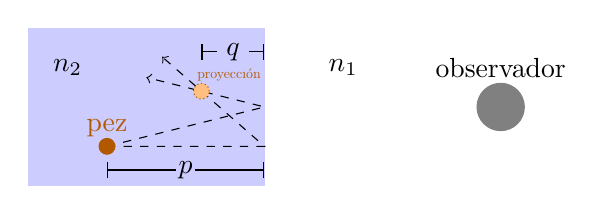
\begin{tikzpicture}
        \filldraw[blue!20] (-2,0) rectangle (1,2);

        \draw[ ->, dashed ] (-1,0.5) -- (1,1) -- (-0.5,1.375);
        \draw[ ->, dashed ] (-1,0.5) -- (1,0.5) -- (-0.3,1.6375);
        \draw[densely dotted, orange!70!black, fill=orange!50] (0.2,1.2) circle (1mm)
        node[yshift=2mm, xshift=3.5mm, scale=0.5] {proyección};

        \filldraw[orange!70!black] (-1,0.5) circle (1mm) node[above] {pez};
        \filldraw[black!50] (4,1) circle (3mm) node[yshift=5mm, color=black] {observador};


        \draw[|-|] (-1, 0.2) -- (1,0.2) node[midway,fill=blue!20,inner sep = 1pt] {$p$};
        \draw[|-|] (0.2, 1.7) -- (1,1.7) node[midway,fill=blue!20] {$q$};

        \draw (-1.5,1.5) node {$n_2$};
        \draw (2,1.5) node {$n_1$};
    \end{tikzpicture}
\end{center}

En este caso, el problema es de dos medios únicamente. Ya que se trata
de un "lente" plano, se puede tomar como un lente esférico cuyo radio
tiende a infinito. Considerando lo obtenido para dos medios:

\[
    \begin{derivation}
            \res{ \frac{n_1 - n_2}{R} = \frac{n_2}{p} + \frac{n_1}{q} }\\
        \why{ $R \to \infty$}\\
            \res{ -\frac{n_2}{p} = \frac{n_1}{q} }\\
        \equiv\\
            \res{ -\frac{n_1}{n_2}p = q }
    \end{derivation}
\]

Ahora, si la distancia del pez al borde de la pecera varía con el
tiempo siguiendo una función $p(t)$, se puede hallar la distancia de la
proyección en ese mismo instante de tiempo mediante una función $q(t)$.
Estas dos funciones se relacionan de la misma forma que las distancias
fijas $p$ y $q$. Así, se puede determinar la velocidad con la que el
pez se distancia del borde de la pecera percibida por el observador.

\[
    \begin{derivation}
            \res{ -\frac{n_1}{n_2}p(t) = q(t) }\\
        \To\\
            \res{ -\frac{n_1}{n_2}p'(t) = q'(t) }
    \end{derivation}
\]

Un ejemplo numérico puede ser: la distancia del pez a la pecera
inicialmente es \qty{10}{\cm}. Luego, la distancia varía siguiendo la
función $p(t) = \sin^2(t) + 10e^{-t}$. Hallar la distancia y velocidad
percibidaa inicialmente y la distancia percibida tras \qty{10}{\s}.

\begin{enumerate}
    \item En el momento inicial:
    Reemplazando en el resultado obtenido:
    \[q_0 = -\frac{1}{1.33}(\qty{10}{\cm}) = \qty{-7.52}{\cm}\]
    El resultado tiene sentido, pues la proyección se produce dentro
    del agua. Por la convención de signos, $q$ debe ser negativo.
    \item En $t = \qty{10}{\s}$
    \[
        \begin{derivation}
            \res{ -\frac{n_1}{n_2}p(t) = q(t) }\\
        \To\\
            \res{
                q(10) = \qty{-2.23e-1}{\cm}\\
                &\land\\
                &q'(t) = -\dfrac{n_1}{n_2}(2\,\sin(t)\cos(t) - 10e^{-t})
            }\\
        \To\\
            \res{
                q(10) = \qty{-2.23e-1}{\cm} \land q'(10) = \qty{-0.6861}{\cm\per\s}
            }
        \end{derivation}  
    \]
\end{enumerate}